% interactnlmsample.tex
% v1.05 - August 2017

\documentclass[dvipdfmx]{interact}
\usepackage{epstopdf}
\usepackage[caption=false]{subfig}

\usepackage{graphics,amsmath,amssymb,bm,float,cases}
\usepackage{here}
\usepackage{comment}
\usepackage{url}
\usepackage{layout}
\usepackage{tabularx}
\usepackage{algorithm}
\usepackage{algorithmic}
\usepackage{xcolor}
\usepackage{multirow}


\usepackage[numbers,sort&compress]{natbib}% Citation support using natbib.sty
\bibpunct[, ]{[}{]}{,}{n}{,}{,}% Citation support using natbib.sty
\renewcommand\bibfont{\fontsize{10}{12}\selectfont}% Bibliography support using natbib.sty
\makeatletter% @ becomes a letter
\def\NAT@def@citea{\def\@citea{\NAT@separator}}% Suppress spaces between citations using natbib.sty
\makeatother% @ becomes a symbol again

\theoremstyle{plain}% Theorem-like structures provided by amsthm.sty
\newtheorem{theorem}{Theorem}[section]
\newtheorem{lemma}[theorem]{Lemma}
\newtheorem{corollary}[theorem]{Corollary}
\newtheorem{proposition}[theorem]{Proposition}
\newtheorem{assumption}{Assumption}

\theoremstyle{definition}
\newtheorem{definition}[theorem]{Definition}
\newtheorem{example}[theorem]{Example}

\theoremstyle{remark}
\newtheorem{remark}{Remark}
\newtheorem{notation}{Notation}


% \newcommand{\Figref}[1]{Figure \ref{#1}}
% \newcommand{\Tabref}[1]{Table \ref{#1}}
% \newcommand{\Eqref}[1]{(Equation \ref{#1})}
% \newcommand{\Secref}[1]{Section \ref{#1}}
% \newcommand{\Theoref}[1]{Theorem \ref{#1}}
\DeclareGraphicsExtensions{.eps,.pdf,.png,.jpg}
\newcommand{\Tabref}[1]{{Table~\ref{#1}}}
\newcommand{\Eqref}[1]{Eq.~(\ref{#1})}
\newcommand{\Figref}[1]{{Fig.~\ref{#1}}}

\begin{document}

\articletype{ARTICLE TEMPLATE}% Specify the article type or omit as appropriate

\title{Probabilistic Multi-Agent Pose Graph Filtering on SE(3) \\ via Distributed ADMM and Stein Particle Gradient Descent}

\author{
\name{Tomoki Arita\textsuperscript{a} and Toru Namerikawa\textsuperscript{b}\thanks{CONTACT Tomoki Arita. Email: arita.tomoki@keio.jp, Toru Namerikawa. Email: namerikawa@sd.keio.ac.jp}}
\affil{\textsuperscript{a} School of Integrated Design Engineering, Keio University, Kanagawa, Japan\\
	\textsuperscript{b} Department of System Design Engineering, Keio University, Kanagawa, Japan}
}

\maketitle

\begin{abstract}
    This paper proposes a novel distributed probabilistic pose graph filtering framework on SE(3). It integrates ADMM with Stein Variational Gradient Descent (SVGD) to address multi-modal, non-Gaussian posteriors in multi-robot SLAM.
    We reformulate pose graph filtering as Bayesian posterior estimation on SE(3) using particles. The consistency requirement, minimizing KL divergence, is cast into an augmented Lagrangian and decomposed via ADMM. Agents perform local SVGD updates and consensus steps, communicating only summary statistics.
    The proposed method (i) maintains multiple hypotheses for ambiguous loop closures, (ii) reduces communication by exchanging only Lagrange multipliers and particle summaries, and (iii) handles SE(3) nonlinearity. Convergence is proven under standard ADMM conditions, and KL minimization is validated.
    Simulations demonstrate real-time convergence, outlier robustness, and accurate posterior approximation.
\end{abstract}

\begin{keywords}
Probabilistic pose graph filtering; SE(3); ADMM; Stein Variational Gradient Descent; Multi-robot SLAM
\end{keywords}

\section{Introduction}
\label{sec:introduction}

Simultaneous Localization and Mapping (SLAM) \cite{Cadena2016} is crucial for autonomous robots. Graph-based SLAM \cite{Grisetti2010}, which formulates SLAM as a nonlinear least-squares problem on SE(3), is standard. Solvers like g2o \cite{Kuemmerle2011} and iSAM2 \cite{Kaess2012} find the Maximum A Posteriori (MAP) estimate. Multi-robot SLAM (MR-SLAM) offers benefits but faces challenges in maintaining global consistency with communication constraints. Distributed architectures, such as those using Distributed Data Fusion SAM (DDF-SAM) \cite{Cunningham2013} or the Alternating Direction Method of Multipliers (ADMM) \cite{Choudhary2015, Boyd2011, Choudhary2017}, have gained prominence. Robustness to outliers, e.g., via DOOR-SLAM \cite{Lajoie2020}, is also critical.
However, MAP-based methods discard uncertainty information and struggle with multimodality. Representing the full posterior is vital. Non-parametric methods like Particle Filters (PFs) \cite{Montemerlo2002} can represent multimodal distributions but scale poorly. This motivates scalable methods for posterior capture.

Our work builds on graph-based SLAM, distributed optimization (ADMM \cite{Boyd2011, Choudhary2015}), non-parametric Bayesian inference (PFs \cite{Montemerlo2002}, SVGD \cite{Liu2016, Pavlasek2023, Koide2024MegaParticles}), probabilistic SLAM (Variational Inference \cite{Cao2024}), and robust estimation \cite{Agarwal2013, Sunderhauf2012, Olson2013, Yang2020, Latif2013, Mangelson2018}.
Traditional robust methods often target MAP estimation; integrating robustness into a fully probabilistic framework that maintains multiple hypotheses is an open challenge.

This paper proposes ADMM-based Stein Particle Filter Probabilistic Graph Filtering (ASP-PGF) for MR-SLAM. It integrates ADMM with SVGD for distributed non-parametric Bayesian inference in pose graph filtering.
Contributions are:
\begin{enumerate}
    \item \textbf{Distributed Non-Parametric Posterior Estimation via ADMM and SVGD Integration:} We formulate MR-SLAM as a distributed posterior estimation task. By integrating ADMM and SVGD, our method achieves globally consistent non-parametric posterior estimation with communication efficiency, where ADMM decomposes the global inference into local SVGD-based subproblems.
    \item \textbf{Robust Multimodal Uncertainty Handling:} The proposed framework explicitly represents complex uncertainties, including non-Gaussianity and multimodality, using SVGD. It inherently handles outliers within the Bayesian inference process, as inconsistent hypotheses are statistically down-weighted or pruned.
\end{enumerate}
This work advances fully probabilistic, distributed MR-SLAM, providing richer information for downstream tasks.

\section{Preliminary}
\label{sec:preliminary}

This section introduces the core mathematical concepts utilized in our proposed method: Stein Variational Gradient Descent (SVGD) for non-parametric Bayesian inference and the Alternating Direction Method of Multipliers (ADMM) for distributed optimization.

\subsection{Stein Variational Gradient Descent (SVGD)}

% \textbf{Theorem 1.} (Stein Variational Gradient Descent \cite{Liu2016})
\begin{theorem}[Stein Variational Gradient Descent \cite{Liu2016}]
\label{thm:svgd}
Let $p(x)$ be a target probability distribution and $q(x)$ be an approximating distribution implicitly represented by a set of particles $\{x_i\}_{i=1}^m$. Let ${\mathcal{H}}^d$ be a Reproducing Kernel Hilbert Space (RKHS) associated with a positive definite kernel $k(x, x')$. The goal is to minimize the Kullback-Leibler (KL) divergence $D_{KL}(q \| p)$ defined in \Eqref{eq:kl_min_prelim}:
\begin{equation}
\begin{aligned}
 q^{*}&=\underset{q \in {\mathcal{Q}}}{\arg\min}\left\{D_{KL}(q \| p) \equiv {{\mathbb{E}}}_{q}[\log q(x)]-{{\mathbb{E}}}_{q}[\log {p}(x)] \right\}.
 \label{eq:kl_min_prelim}
\end{aligned}
\end{equation}
The direction ${\boldsymbol{\Phi}}_{q, p}^{*} \in {\mathcal{H}}^d$ that maximally decreases the KL divergence within the unit ball of the RKHS, i.e., maximizes ${{\mathbb{E}}}_{x \sim q}\left[{\mathcal{A}}_{p} {\boldsymbol{\Phi}}(x)\right]$ subject to $\|{\boldsymbol{\Phi}}\|_{{\mathcal{H}}^d} \leq 1$, is given by:
\begin{equation}
\begin{aligned}
{\boldsymbol{\Phi}}_{q, p}^{*}(x') = {{\mathbb{E}}}_{x \sim q}\left[k(x, x') \nabla_{x} \log p(x) + \nabla_{x} k(x, x')\right].
\label{eq:phi_solution_prelim}
\end{aligned}
\end{equation}
Here, ${\mathcal{A}}_{p}$ is the Stein operator defined as:
\begin{equation}
\begin{aligned}
{\mathcal{A}}_{p} {\boldsymbol{\Phi}}(x) = \nabla_{x} \log p(x)^{\top} {\boldsymbol{\Phi}}(x) + \nabla_{x} \cdot {\boldsymbol{\Phi}}(x).
\label{eq:stein_operator}
\end{aligned}
\end{equation}
The maximum decrease rate is related to the Kernelized Stein Discrepancy (KSD):
\begin{equation}
\begin{aligned}
{{\mathbb{D}}}(q,p)&=\max_{{\boldsymbol{\Phi}}\in {\mathcal{H}}^d, \|{\boldsymbol{\Phi}}\|_{{\mathcal{H}}^d} \leq 1}{{\mathbb{E}}}_{x \sim q}\left[{\mathcal{A}}_{p} {\boldsymbol{\Phi}}(x)\right] = \|{\boldsymbol{\Phi}}_{q, p}^{*}\|_{{\mathcal{H}}^d}.
\label{eq:ksd_prelim}
\end{aligned}
\end{equation}
\end{theorem}

% \textit{Practical Implementation.}
In practice, the expectation in \Eqref{eq:phi_solution_prelim} is approximated using the empirical distribution of the particles 
$q(x) \approx \frac{1}{m} \sum_{i=1}^m \delta(x - x_i)$. 
The update rule for each particle $x_l$ becomes a deterministic step in the direction ${\boldsymbol{\Phi}}^{*}(x_l)$:
\begin{equation}
\begin{aligned}
x_l \leftarrow x_l + \epsilon {\boldsymbol{\Phi}}^{*}(x_l),
\label{eq:svgd_update_rule}
\end{aligned}
\end{equation}
where $\epsilon$ is a step size and ${\boldsymbol{\Phi}}^{*}(x_l)$ is the empirical estimate of the optimal direction:
\begin{equation}
\begin{aligned}
{\boldsymbol{\Phi}}^{*}(x_l) = \frac{1}{m}\sum_{i=1}^m \left[ k(x_i, x_l) \nabla_{x_i} \log p(x_i) + \nabla_{x_i} k(x_i, x_l) \right].
\label{eq:svgd_practical_update}
\end{aligned}
\end{equation}
This update drives the particles towards the target distribution $p(x)$ by balancing two terms: the first term pushes particles towards high-probability regions of $p(x)$, while the second term acts as a repulsive force between particles, encouraging diversity and preventing collapse to a single mode.

\subsection{Alternating Direction Method of Multipliers (ADMM)}
\label{subsec:admm}

The Alternating Direction Method of Multipliers (ADMM) \cite{Boyd2011} is an algorithm for solving convex optimization problems, particularly those that can be decomposed into smaller subproblems. It is well-suited for distributed consensus problems. Consider the problem of minimizing a sum of local objective functions $f_i(x_i)$ subject to a consensus constraint $x_i = z$ for all agents $i=1, \dots, N$:
\begin{equation}
\begin{aligned}
\min_{x_1, \dots, x_N} & \sum_{i=1}^N f_i(x_i) \\
\text{s.t.} \quad & x_i - z = 0, \quad \forall i.
\label{eq:admm_consensus_problem_prelim}
\end{aligned}
\end{equation}
ADMM utilizes the augmented Lagrangian ${\mathcal{L}}_{\rho}$:
\begin{equation}
\begin{aligned}
{\mathcal{L}}_{\rho}(\{x_i\}, z, \{\lambda_i\}) = \sum_{i=1}^N \left( f_i(x_i) + \lambda_i^{\top} (x_i - z) + \frac{\rho}{2} \|x_i - z\|^2 \right),
\label{eq:admm_augmented_lagrangian_prelim}
\end{aligned}
\end{equation}
where $\lambda_i$ are dual variables and $\rho > 0$ is a penalty parameter. The algorithm iteratively updates the primal variables ($x_i$, $z$) and dual variables ($\lambda_i$) at iteration $k+1$ as follows:
\begin{equation}
\begin{aligned}
x_i^{k+1} &= \underset{x_i}{\arg\min} {\mathcal{L}}_{\rho}(x_i, z^k, \lambda_i^k), \quad \forall i \\
z^{k+1} &= \underset{z}{\arg\min} {\mathcal{L}}_{\rho}(\{x_i^{k+1}\}, z, \{\lambda_i^k\}) \\
\lambda_i^{k+1} &= \lambda_i^k + \rho (x_i^{k+1} - z^{k+1}), \quad \forall i.
\label{eq:admm_updates_prelim}
\end{aligned}
\end{equation}
The $x$-updates can often be performed in parallel by each agent. The $z$-update typically involves gathering information from all agents (e.g., averaging). The dual update is also performed locally. These steps are repeated until convergence. ADMM combines the decomposability of dual ascent with the robust convergence of the method of multipliers.
While ADMM is traditionally analyzed for convex problems, its application to non-convex problems has also been explored, often with convergence guarantees to local optima or stationary points under certain conditions \cite{Hong2016, Wang2019}. In such non-convex settings, the choice of penalty parameter $\rho$ and initialization can significantly impact performance and convergence. Our work leverages ADMM in a non-convex pose graph setting, where the underlying problem involves SE(3) manifolds.

\section{Problem Formulation}
\label{sec:problem_formulation}

This section formally defines the multi-agent pose graph filtering problem addressed in this paper. We begin by establishing the notation used for representing poses and transformations on the Special Euclidean group SE(3), followed by the deterministic and probabilistic formulations of the pose graph filtering problem.

\subsection{Notation on SE(3)}
\label{subsec:notation_se3}

We represent the state (pose) of an agent $i$ at time $t$ as an element of the Special Euclidean group SE(3), denoted by $X_i^t \in \text{SE}(3)$. SE(3) is the group of rigid body transformations in three-dimensional space, combining rotation and translation. An element $X \in \text{SE}(3)$ can be represented by a $4 \times 4$ homogeneous transformation matrix:
\begin{equation}
\begin{aligned}
X =
\begin{pmatrix}
{\mathbf{R}} & {\mathbf{t}} \\
{\mathbf{0}}^{\top} & 1
\end{pmatrix} \in {\mathbb{R}}^{4\times4},
\label{eq:se3_matrix_form}
\end{aligned}
\end{equation}
where ${\mathbf{R}} \in \text{SO}(3)$ is a $3 \times 3$ rotation matrix representing the orientation, and ${\mathbf{t}} \in {\mathbb{R}}^3$ is the translation vector representing the position. SO(3) is the Special Orthogonal group, the space of $3 \times 3$ orthogonal matrices with determinant +1.

The Lie algebra associated with SE(3) is denoted by ${\mathfrak{se}}(3)$. It is the tangent space to the identity element of SE(3) and represents infinitesimal transformations (velocities). An element $\boldsymbol{\xi} \in {\mathfrak{se}}(3)$ is a 6-dimensional vector, often called a twist, composed of translational and rotational velocity components: $\boldsymbol{\xi} = (\boldsymbol{\nu}^{\top}, \boldsymbol{\omega}^{\top})^{\top}$, where $\boldsymbol{\nu} \in {\mathbb{R}}^3$ is the translational velocity and $\boldsymbol{\omega} \in {\mathbb{R}}^3$ is the rotational velocity.

We use the hat operator $(\cdot)^{\wedge}$ to map elements from the vector space ${\mathbb{R}}^6$ to the Lie algebra ${\mathfrak{se}}(3)$ represented as $4 \times 4$ matrices:
\begin{equation}
\begin{aligned}
\boldsymbol{\xi}^{\wedge} =
\begin{pmatrix}
\boldsymbol{\omega}^{\wedge} & \boldsymbol{\nu} \\
{\mathbf{0}}^{\top} & 0
\end{pmatrix} \in {\mathbb{R}}^{4\times4},
\label{eq:se3_hat_operator}
\end{aligned}
\end{equation}
where $\boldsymbol{\omega}^{\wedge}$ is the skew-symmetric matrix corresponding to the rotational velocity vector $\boldsymbol{\omega} \in {\mathbb{R}}^3$:
\begin{equation}
\begin{aligned}
\boldsymbol{\omega}^{\wedge} =
\begin{pmatrix}
0 & -\omega_z & \omega_y \\
\omega_z & 0 & -\omega_x \\
-\omega_y & \omega_x & 0
\end{pmatrix} \in {\mathfrak{so}}(3).
\label{eq:so3_hat_operator}
\end{aligned}
\end{equation}
Here, ${\mathfrak{so}}(3)$ is the Lie algebra of SO(3).

The exponential map $\exp: {\mathfrak{se}}(3) \to \text{SE}(3)$ maps an element from the Lie algebra to the Lie group. For $\boldsymbol{\xi} = (\boldsymbol{\nu}^{\top}, \boldsymbol{\omega}^{\top})^{\top} \in {\mathfrak{se}}(3)$, the exponential map is given by:
\begin{equation}
\begin{aligned}
\exp(\boldsymbol{\xi}^{\wedge}) =
\begin{pmatrix}
\exp(\boldsymbol{\omega}^{\wedge}) & {\mathbf{V}}(\boldsymbol{\omega}) \boldsymbol{\nu} \\
{\mathbf{0}}^{\top} & 1
\end{pmatrix} \in \text{SE}(3),
\label{eq:se3_exp_map}
\end{aligned}
\end{equation}
where $\exp(\boldsymbol{\omega}^{\wedge}) \in \text{SO}(3)$ is the matrix exponential for rotations (Rodrigues' formula), and ${\mathbf{V}}(\boldsymbol{\omega})$ is a $3 \times 3$ matrix:
\begin{equation}
\begin{aligned}
\exp(\boldsymbol{\omega}^{\wedge}) &= {\mathbf{I}}_3 + \frac{\sin \theta}{\theta } \boldsymbol{\omega}^{\wedge} + \frac{1-\cos \theta }{\theta^2}(\boldsymbol{\omega}^{\wedge})^2, \\
{\mathbf{V}}(\boldsymbol{\omega}) &= {\mathbf{I}}_3 + \frac{1-\cos\theta}{\theta^2}\boldsymbol{\omega}^{\wedge} + \frac{\theta-\sin \theta}{\theta^3}(\boldsymbol{\omega}^{\wedge})^2,
\label{eq:so3_exp_and_V}
\end{aligned}
\end{equation}
with $\theta = \|\boldsymbol{\omega}\|$.

The inverse operation, the logarithm map $\log: \text{SE}(3) \to {\mathfrak{se}}(3)$, maps an element from the group back to the algebra. The vee operator $(\cdot)^{\vee}$ maps elements from the matrix representation of the Lie algebra back to the vector space ${\mathbb{R}}^6$. These operations allow us to represent differences between poses in the tangent space. For two poses $X_1, X_2 \in \text{SE}(3)$, their relative transformation is $X_{12} = X_1^{-1} X_2$. The difference in the tangent space at the identity is $\boldsymbol{\xi}_{12} = (\log(X_{12}))^{\vee}$.

\subsection{Probabilistic Problem Formulation for PGF}
\label{subsec:probabilistic_pgo}

The Pose Graph Filtering (PGF) problem aims to estimate the set of poses ${\mathbf{X}} = \{X_i\}_{i \in {\mathcal{V}}}$ for a collection of agents or time steps (nodes ${\mathcal{V}}$ in the graph), given a set of relative pose measurements ${\tilde{Z}}_{ij}$ between pairs of poses $(i, j) \in {\mathcal{E}}$ (edges ${\mathcal{E}}$ in the graph). These measurements typically come from odometry or loop closures. Each measurement ${\tilde{Z}}_{ij} \in \text{SE}(3)$ represents the measured transformation from pose $X_i$ to pose $X_j$. The error $E_{ij}(X_i, X_j) = {\tilde{Z}}_{ij}^{-1} (X_i^{-1} X_j)$ represents the discrepancy.

From a probabilistic perspective, PGF aims to estimate the posterior $P({\mathbf{X}} | {\mathbf{Z}})$ 
of poses${\mathbf{X}}$ given measurements ${\mathbf{Z}} = \{{\tilde{Z}}_{ij}\}$. Assuming independent Gaussian errors $\log(E_{ij}(X_i,X_j))^{\vee} \sim {\mathcal{N}}({\mathbf{0}}, \Sigma_{ij})$, the likelihood $P({\tilde{Z}}_{ij} | X_i, X_j) \propto \exp( -\frac{1}{2} \| \log({\tilde{Z}}_{ij}^{-1} X_i^{-1} X_j)^{\vee} \|^2_{\Omega_{ij}} )$.
The total likelihood is $P({\mathbf{Z}} | {\mathbf{X}}) = \prod P({\tilde{Z}}_{ij} | X_i, X_j)$.
By Bayes' theorem, $P({\mathbf{X}} | {\mathbf{Z}}) \propto P({\mathbf{Z}} | {\mathbf{X}}) P({\mathbf{X}})$.
The Maximum A Posteriori (MAP) estimate ${\mathbf{X}}^*_{MAP}$ maximizes $P({\mathbf{X}} | {\mathbf{Z}})$, or equivalently minimizes:
\begin{equation}
\begin{aligned}
J_{MAP}({\mathbf{X}}) = \frac{1}{2} \sum_{(i,j) \in {\mathcal{E}}} \| \log({\tilde{Z}}_{ij}^{-1} X_i^{-1} X_j)^{\vee} \|^2_{\Omega_{ij}} - \log P({\mathbf{X}}).
\label{eq:map_estimation_min_pgf}
\end{aligned}
\end{equation}
With a uniform prior $P({\mathbf{X}})$, this reduces to a nonlinear least-squares problem.
Standard PGF finds the posterior mode, discarding uncertainty. A more general approach approximates the full posterior $P({\mathbf{X}} | {\mathbf{Z}})$ by finding $q({\mathbf{X}})$ that minimizes the Kullback-Leibler (KL) divergence:
\begin{equation}
\begin{aligned}
q^*({\mathbf{X}}) = \underset{q \in {\mathcal{Q}}}{\arg\min} \, D_{KL}(q({\mathbf{X}}) \| P({\mathbf{X}} | {\mathbf{Z}})).
\label{eq:kl_min_objective}
\end{aligned}
\end{equation}
Minimizing the KL divergence is equivalent to minimizing the variational free energy ${\mathcal{F}}[q]$ (since the evidence $P({\mathbf{Z}})$ is constant w.r.t. $q$):
\begin{equation}
\begin{aligned}
D_{KL}(q \| P) % &= \int q({\mathbf{X}}) \log \frac{q({\mathbf{X}})}{P({\mathbf{X}} | {\mathbf{Z}})} d{\mathbf{X}} \\
% &= -{\mathcal{H}}[q] + \mathbb{E}_q[-\log P({\mathbf{Z}} | {\mathbf{X}}) - \log P({\mathbf{X}})] + \log P({\mathbf{Z}}) \\
&= {\mathcal{F}}[q] + \log P({\mathbf{Z}}), \\
\text{where} \quad {\mathcal{F}}[q] &= \mathbb{E}_q[-\log P({\mathbf{Z}} | {\mathbf{X}}) - \log P({\mathbf{X}})] - {\mathcal{H}}[q].
\label{eq:kl_free_energy}
\end{aligned}
\end{equation}
Here, ${\mathcal{H}}[q] = -\int q({\mathbf{X}}) \log q({\mathbf{X}}) d{\mathbf{X}}$ is the entropy of the distribution $q$. Assuming a uniform prior $P({\mathbf{X}})$ and using the likelihood definition described earlier (leading to the MAP formulation in \Eqref{eq:map_estimation_min_pgf}), the term $-\log P({\mathbf{Z}} | {\mathbf{X}})$ corresponds to the PGF cost function (up to constants):
\begin{equation}
\begin{aligned}
C({\mathbf{X}}) = \frac{1}{2} \sum_{(i,j) \in {\mathcal{E}}} \| \log({\tilde{Z}}_{ij}^{-1} X_i^{-1} X_j)^{\vee} \|^2_{\Omega_{ij}}.
\label{eq:cost_function_C}
\end{aligned}
\end{equation}
Thus, minimizing the KL divergence becomes equivalent to minimizing the free energy, which involves a trade-off between minimizing the expected cost and maximizing the entropy:
\begin{equation}
\begin{aligned}
\min_q {\mathcal{F}}[q] = \min_q \left( \mathbb{E}_q[C({\mathbf{X}})] - {\mathcal{H}}[q] \right).
\label{eq:kl_min_cost_entropy}
\end{aligned}
\end{equation}
This formulation seeks a distribution $q$ that concentrates on low-cost configurations (low $\mathbb{E}_q[C({\mathbf{X}})]$) while maximizing entropy ${\mathcal{H}}[q]$ (representing uncertainty).

% The standard MAP estimation \Eqref{eq:map_estimation_min_pgf} can be recovered as a special case of this KL minimization framework. If we restrict the approximating distribution $q({\mathbf{X}})$ to be a Dirac delta function centered at a single point ${\mathbf{X}}_0$, i.e., $q({\mathbf{X}}) = \delta({\mathbf{X}} - {\mathbf{X}}_0)$, then the entropy term ${\mathcal{H}}[q]$ becomes negative infinity (or is undefined, but its contribution vanishes in the limit). The expectation $\mathbb{E}_q[C({\mathbf{X}})]$ simply evaluates the cost function at ${\mathbf{X}}_0$, i.e., $\mathbb{E}_q[C({\mathbf{X}})] = C({\mathbf{X}}_0)$. In this case, minimizing the free energy (ignoring the problematic entropy term) reduces to minimizing $C({\mathbf{X}}_0)$, which is exactly the deterministic PGF problem \Eqref{eq:deterministic_pgf_final} (equivalent to MAP estimation with a uniform prior). Therefore, the deterministic formulation finds a single point estimate by implicitly using a Dirac delta approximation within the broader probabilistic framework of KL divergence minimization. Our work, detailed in the following sections, focuses on using more expressive non-parametric distributions for $q({\mathbf{X}})$ to capture the full posterior uncertainty.

\section{Probabilistic Multi-Agent Pose Graph Filtering on SE(3)}
\label{sec:probabilistic_pgf}

As established in Section \ref{subsec:probabilistic_pgo}, our goal is to approximate the full posterior distribution $P({\mathbf{X}} | {\mathbf{Z}})$ by finding a distribution $q({\mathbf{X}})$ that minimizes the KL divergence $D_{KL}(q({\mathbf{X}}) \| P({\mathbf{X}} | {\mathbf{Z}}))$, which is equivalent to minimizing the variational free energy ${\mathcal{F}}[q] = \mathbb{E}_q[C({\mathbf{X}})] - {\mathcal{H}}[q]$ under a uniform prior assumption (\Eqref{eq:kl_min_cost_entropy}). This section details our approach to solving this minimization problem in a distributed multi-agent setting using a mean-field approximation and ADMM combined with SVGD.

\subsection{Mean-Field Factorization of the Joint Posterior}
\label{subsec:mean_field}

The joint posterior distribution $P({\mathbf{X}} | {\mathbf{Z}})$ over all poses ${\mathbf{X}} = \{X_i\}_{i \in {\mathcal{V}}}$ is generally high-dimensional and complex, making direct minimization of \Eqref{eq:kl_min_cost_entropy} intractable. To make the problem computationally feasible, particularly in a distributed setting, we employ a mean-field approximation. We assume that the approximating distribution $q({\mathbf{X}})$ factorizes over the individual poses (nodes in the graph):
\begin{equation}
\begin{aligned}
q({\mathbf{X}}) \approx \prod_{i \in {\mathcal{V}}} q_i(X_i),
\label{eq:mean_field_approx}
\end{aligned}
\end{equation}
where each $q_i(X_i)$ is a distribution over the pose $X_i$ of node $i$. This factorization assumes independence between the poses in the approximating distribution, simplifying the optimization.

Under the mean-field assumption, the entropy term decomposes additively:
\begin{equation}
\begin{aligned}
{\mathcal{H}}[q] &= -\int q({\mathbf{X}}) \log q({\mathbf{X}}) d{\mathbf{X}} \\
&= -\int \prod_k q_k(X_k) \sum_i \log q_i(X_i) d{\mathbf{X}} \\
&= -\sum_i \int q_i(X_i) \log q_i(X_i) dX_i \prod_{k \neq i} \int q_k(X_k) dX_k \\
&= \sum_{i \in {\mathcal{V}}} {\mathcal{H}}[q_i].
\label{eq:entropy_mean_field}
\end{aligned}
\end{equation}
The expected cost term becomes:
\begin{equation}
\begin{aligned}
\mathbb{E}_q[C({\mathbf{X}})] &= \mathbb{E}_q \left[ \sum_{(i,j) \in {\mathcal{E}}} c_{ij}(X_i, X_j) \right] \\
% &= \sum_{(i,j) \in {\mathcal{E}}} \mathbb{E}_q [c_{ij}(X_i, X_j)] \\
&= \sum_{(i,j) \in {\mathcal{E}}} \iint c_{ij}(X_i, X_j) q_i(X_i) q_j(X_j) dX_i dX_j,
\label{eq:expected_cost_mean_field}
\end{aligned}
\end{equation}
where $c_{ij}(X_i, X_j) = \frac{1}{2} \| \log({\tilde{Z}}_{ij}^{-1} X_i^{-1} X_j)^{\vee} \|^2_{\Omega_{ij}}$.

Substituting these into the free energy minimization \Eqref{eq:kl_min_cost_entropy}, the objective becomes:
\begin{equation}
\begin{aligned}
\min_{q_1, \dots, q_N} \left( \sum_{(i,j) \in {\mathcal{E}}} \mathbb{E}_{q_i, q_j}[c_{ij}(X_i, X_j)] - \sum_{i \in {\mathcal{V}}} {\mathcal{H}}[q_i] \right).
\label{eq:kl_min_mean_field}
\end{aligned}
\end{equation}
This objective involves minimizing the expected sum of pairwise costs minus the sum of individual entropies. While simpler than the original problem, directly optimizing \Eqref{eq:kl_min_mean_field} with respect to the distributions $q_i$ is still challenging. The coupling between $q_i$ and $q_j$ in the expectation term $\mathbb{E}_{q_i, q_j}[c_{ij}(X_i, X_j)]$ prevents straightforward independent updates for each $q_i$.

To address this coupling and enable distributed optimization, we will employ ADMM, as detailed in the next subsection. The core idea is to introduce auxiliary variables and constraints to decouple the pairwise expectations, allowing for iterative updates of the individual $q_i$ distributions using SVGD.

\subsection{ADMM Updates for Distributed KL Minimization}
\label{subsec:admm_updates}

To solve the mean-field KL minimization problem \Eqref{eq:kl_min_mean_field} in a distributed manner, we apply the Alternating Direction Method of Multipliers (ADMM). The coupling between $q_i$ and $q_j$ occurs in the expected cost term $\mathbb{E}_{q_i, q_j}[c_{ij}(X_i, X_j)]$. We introduce auxiliary variables $\zeta_{ij}$ for each edge $(i,j) \in {\mathcal{E}}$ to represent these expected values:
\begin{equation}
\begin{aligned}
\zeta_{ij} = \mathbb{E}_{q_i, q_j}[c_{ij}(X_i, X_j)] = \iint c_{ij}(X_i, X_j) q_i(X_i) q_j(X_j) dX_i dX_j.
\label{eq:aux_variable_zeta}
\end{aligned}
\end{equation}
With these auxiliary variables, the optimization problem \Eqref{eq:kl_min_mean_field} can be rewritten as a constrained optimization problem:
\begin{equation}
\begin{aligned}
\min_{q_1, \dots, q_N, \{\zeta_{ij}\}} & \left( \sum_{(i,j) \in {\mathcal{E}}} \zeta_{ij} - \sum_{i \in {\mathcal{V}}} {\mathcal{H}}[q_i] \right) \\
\text{s.t.} \quad & \zeta_{ij} = \mathbb{E}_{q_i, q_j}[c_{ij}(X_i, X_j)], \quad \forall (i,j) \in {\mathcal{E}}.
\label{eq:kl_min_constrained}
\end{aligned}
\end{equation}
The augmented Lagrangian ${\mathcal{L}}_{\rho}$ for this problem is:
\begin{equation}
\begin{aligned}
{\mathcal{L}}_{\rho}(\{q_i\}, \{\zeta_{ij}\}, \{\lambda_{ij}\}) = & \sum_{(i,j) \in {\mathcal{E}}} \zeta_{ij} - \sum_{i \in {\mathcal{V}}} {\mathcal{H}}[q_i] + \sum_{(i,j) \in {\mathcal{E}}} \lambda_{ij} (\zeta_{ij} - \mathbb{E}_{q_i, q_j}[c_{ij}]) \\
& + \frac{\rho}{2} \sum_{(i,j) \in {\mathcal{E}}} (\zeta_{ij} - \mathbb{E}_{q_i, q_j}[c_{ij}])^2,
\label{eq:admm_kl_lagrangian}
\end{aligned}
\end{equation}
where $\lambda_{ij}$ are the dual variables and $\rho > 0$ is the penalty parameter. Note that $\mathbb{E}_{q_i, q_j}[c_{ij}]$ is shorthand for the integral in \Eqref{eq:aux_variable_zeta}.

The ADMM algorithm proceeds by iteratively minimizing ${\mathcal{L}}_{\rho}$ with respect to $\zeta_{ij}$ and $q_i$, followed by an update of the dual variables $\lambda_{ij}$.

\textbf{1. $\zeta$-update:} Minimize ${\mathcal{L}}_{\rho}$ with respect to $\zeta_{ij}$ for all edges $(i,j) \in {\mathcal{E}}$, keeping $q_i$ and $\lambda_{ij}$ fixed.
\begin{equation}
\begin{aligned}
\zeta_{ij}^{k+1} = \underset{\zeta_{ij}}{\arg\min} & \left( \zeta_{ij} + \lambda_{ij}^k (\zeta_{ij} - \mathbb{E}_{q_i^k, q_j^k}[c_{ij}]) + \frac{\rho}{2} (\zeta_{ij} - \mathbb{E}_{q_i^k, q_j^k}[c_{ij}])^2 \right).
\label{eq:admm_zeta_update_min}
\end{aligned}
\end{equation}
Taking the derivative with respect to $\zeta_{ij}$ and setting it to zero:
\begin{equation}
\begin{aligned}
1 + \lambda_{ij}^k + \rho (\zeta_{ij} - \mathbb{E}_{q_i^k, q_j^k}[c_{ij}]) = 0.
\label{eq:admm_zeta_deriv}
\end{aligned}
\end{equation}
Solving for $\zeta_{ij}$ yields the update:
\begin{equation}
\begin{aligned}
\zeta_{ij}^{k+1} = \mathbb{E}_{q_i^k, q_j^k}[c_{ij}] - \frac{1 + \lambda_{ij}^k}{\rho}.
\label{eq:admm_zeta_update}
\end{aligned}
\end{equation}
This step can be performed locally for each edge.

\textbf{2. $q$-update:} Minimize ${\mathcal{L}}_{\rho}$ with respect to each $q_i$ for all nodes $i \in {\mathcal{V}}$, keeping $\zeta_{ij}$ and $\lambda_{ij}$ fixed at their latest values ($\zeta_{ij}^{k+1}, \lambda_{ij}^k$). The terms involving $q_i$ define the local objective function ${\mathcal{L}}_{\rho, i}$ for agent $i$:
\begin{equation}
\begin{aligned}
q_i^{k+1} = \underset{q_i}{\arg\min} & \underbrace{\left( -{\mathcal{H}}[q_i] + \sum_{j \in {\mathcal{N}}_i} \left[ \lambda_{ij}^k (\zeta_{ij}^{k+1} - \mathbb{E}_{q_i, q_j^k}[c_{ij}]) + \frac{\rho}{2} (\zeta_{ij}^{k+1} - \mathbb{E}_{q_i, q_j^k}[c_{ij}])^2 \right] \right)}_{\text{Objective for } q_i: {\mathcal{L}}_{\rho, i}},
\label{eq:admm_q_update_min}
\end{aligned}
\end{equation}
where ${\mathcal{N}}_i$ denotes the neighbors of node $i$ in the graph. Taking the functional derivative of ${\mathcal{L}}_{\rho, i}$ with respect to $q_i(X_i)$ and setting it to zero (using $\nabla_{q_i} {\mathcal{H}}[q_i] = -1 - \log q_i(X_i)$ and $\nabla_{q_i} \mathbb{E}_{q_i, q_j^k}[c_{ij}] = \int c_{ij}(X_i, X_j) q_j^k(X_j) dX_j = \bar{c}_{ij}(X_i)$):
\begin{equation}
\begin{aligned}
\nabla_{q_i} {\mathcal{L}}_{\rho, i} = & -(-1 - \log q_i(X_i)) + \sum_{j \in {\mathcal{N}}_i} [-\lambda_{ij}^k - \rho(\zeta_{ij}^{k+1} - \mathbb{E}_{q_i, q_j^k}[c_{ij}])] \nabla_{q_i} \mathbb{E}_{q_i, q_j^k}[c_{ij}] \\
= & 1 + \log q_i(X_i) + \sum_{j \in {\mathcal{N}}_i} [-\lambda_{ij}^k - \rho(\zeta_{ij}^{k+1} - \mathbb{E}_{q_i, q_j^k}[c_{ij}])] \bar{c}_{ij}(X_i) = 0.
\label{eq:admm_q_deriv}
\end{aligned}
\end{equation}
This equation implicitly defines the optimal $q_i^{k+1}$. Rearranging gives:
\begin{equation}
\begin{aligned}
\log q_i^{k+1}(X_i) \propto \sum_{j \in {\mathcal{N}}_i} [\lambda_{ij}^k + \rho(\zeta_{ij}^{k+1} - \mathbb{E}_{q_i, q_j^k}[c_{ij}])] \bar{c}_{ij}(X_i).
\label{eq:admm_q_solution_form}
\end{aligned}
\end{equation}
Finding $q_i^{k+1}$ directly is difficult. However, the condition $\nabla_{q_i} {\mathcal{L}}_{\rho, i} = 0$ implies that the update step aims to find a distribution $q_i$ such that its log-density matches the derived expression. This is equivalent to minimizing the KL divergence $D_{KL}(q_i \| q_i^*)$, where $q_i^*$ is the (unnormalized) target distribution defined by the right-hand side of \Eqref{eq:admm_q_solution_form}.
We can solve this KL minimization problem using SVGD. The SVGD update for particles $\{X_{i,l}\}_{l=1}^m$ representing $q_i$ aims to drive them towards $q_i^*$:
\begin{equation}
\begin{aligned}
X_{i,l} \leftarrow X_{i,l} \exp(\epsilon \boldsymbol{\Phi}_i^*(X_{i,l})),
\label{eq:admm_svgd_update}
\end{aligned}
\end{equation}
where the update direction $\boldsymbol{\Phi}_i^*$ is calculated using \Eqref{eq:svgd_practical_update} with the target log-density gradient $\nabla_{X_i} \log q_i^*(X_i)$:
\begin{equation}
\begin{aligned}
\nabla_{X_i} \log q_i^*(X_i) \approx \sum_{j \in {\mathcal{N}}_i} W_{ij}^k \, \mathbb{E}_{q_j^k}[\nabla_{X_i} c_{ij}(X_i, X_j)],
\label{eq:admm_target_gradient}
\end{aligned}
\end{equation}
where $W_{ij}^k = \lambda_{ij}^k + \rho(\zeta_{ij}^{k+1} - \mathbb{E}_{q_i^k, q_j^k}[c_{ij}])$ acts as a weight, and the expectation $\mathbb{E}_{q_j^k}[\cdot]$ is approximated using the particles of agent $j$. The gradient $\nabla_{X_i} c_{ij}(X_i, X_j)$ is required for the SVGD update. Following standard practices in PGO, we approximate this gradient using the Gauss-Newton method on the SE(3) manifold. Specifically, we compute the gradient of the cost term $c_{ij}(X_i, X_j) = \frac{1}{2} \| {\mathbf{r}}_{ij}(X_i, X_j)^\vee \|^2_{\Omega_{ij}}$, where ${\mathbf{r}}_{ij}(X_i, X_j) = \log({\tilde{Z}}_{ij}^{-1} X_i^{-1} X_j)$, with respect to a perturbation $\boldsymbol{\xi} \in {\mathfrak{se}}(3)$ applied to $X_i$ (i.e., $X_i \exp(\boldsymbol{\xi}^\wedge)$). The gradient is approximated as:
\begin{equation}
\begin{aligned}
\nabla_{X_i} c_{ij}(X_i, X_j) &\approx ({\mathbf{H}}_{ij})^{-1} {\mathbf{b}}_{ij}, \\
\text{where} \quad {\mathbf{H}}_{ij} &= ({\mathbf{J}}_{ij})^\top \Omega_{ij} {\mathbf{J}}_{ij}, \\
{\mathbf{b}}_{ij} &= -({\mathbf{J}}_{ij})^\top \Omega_{ij} {\mathbf{r}}_{ij}(X_i, X_j)^\vee, \\
{\mathbf{J}}_{ij} &= \left. \frac{\partial ({\mathbf{r}}_{ij}(X_i \exp(\boldsymbol{\xi}^\wedge), X_j)^\vee)}{\partial \boldsymbol{\xi}} \right|_{\boldsymbol{\xi}=\mathbf{0}}.
\label{eq:gradient_cij_gauss_newton}
\end{aligned}
\end{equation}
Here, ${\mathbf{J}}_{ij}$ is the Jacobian of the residual vector ${\mathbf{r}}_{ij}^\vee$ with respect to the perturbation $\boldsymbol{\xi}$ evaluated at $\boldsymbol{\xi}=\mathbf{0}$. The derivation and explicit form of this Jacobian on SE(3) can be found in standard literature, for example, in the tutorial by Blanco \cite{Blanco2012ATO}. The term $({\mathbf{H}}_{ij})^{-1} {\mathbf{b}}_{ij}$ represents the update step in the tangent space at $X_i$ derived from the Gauss-Newton approximation. This gradient is then used within the SVGD update \Eqref{eq:admm_svgd_update} via \Eqref{eq:admm_target_gradient}.

\textbf{3. $\lambda$-update:} Update the dual variables based on the residual:
\begin{equation}
\begin{aligned}
\lambda_{ij}^{k+1} = \lambda_{ij}^k + \rho (\zeta_{ij}^{k+1} - \mathbb{E}_{q_i^{k+1}, q_j^{k+1}}[c_{ij}]).
\label{eq:admm_lambda_update_kl}
\end{aligned}
\end{equation}
This step requires re-evaluating the expectation with the updated distributions $q_i^{k+1}$.

These three steps constitute one iteration of the ADMM algorithm for distributed KL minimization. By iterating these updates, the individual distributions $q_i$ converge towards a state that minimizes the global KL divergence under the mean-field assumption, effectively approximating the joint posterior $P({\mathbf{X}} | {\mathbf{Z}})$. The overall procedure is summarized in Algorithm \ref{alg:admm_svgd_pgf}.

\begin{algorithm}[H]
\caption{Distributed Probabilistic PGF via ADMM and SVGD (ASP-PGF)}
\label{alg:admm_svgd_pgf}
\begin{algorithmic}[1]
\STATE \textbf{Input:} Pose graph $({\mathcal{V}}, {\mathcal{E}})$, measurements $\{{\tilde{Z}}_{ij}, \Omega_{ij}\}_{(i,j) \in {\mathcal{E}}}$, number of particles $m$, ADMM parameter $\rho$, SVGD step size $\epsilon$.
\STATE \textbf{Initialize:} For each node $i \in {\mathcal{V}}$, initialize particle set $\{X_{i,l}^0\}_{l=1}^m$ representing $q_i^0$. Initialize dual variables $\lambda_{ij}^0 = 0$ for all $(i,j) \in {\mathcal{E}}$. Set iteration counter $k=0$.
\REPEAT
    \STATE \textbf{// $\zeta$-update (for each edge $(i,j) \in {\mathcal{E}}$ in parallel)}
    \STATE Compute $\mathbb{E}_{q_i^k, q_j^k}[c_{ij}]$ using current particles $\{X_{i,l}^k\}, \{X_{j,l}^k\}$.
    \STATE Update $\zeta_{ij}^{k+1} = \mathbb{E}_{q_i^k, q_j^k}[c_{ij}] - (1 + \lambda_{ij}^k)/\rho$ using \Eqref{eq:admm_zeta_update}.
    \STATE \textbf{// $q$-update (for each node $i \in {\mathcal{V}}$ in parallel)}
    \STATE Compute target gradient $\nabla_{X_i} \log q_i^*(X_i)$ using \Eqref{eq:admm_target_gradient}, approximating expectations and gradients using particles $\{X_{j,l}^k\}_{j \in {\mathcal{N}}_i}$ and \Eqref{eq:gradient_cij_gauss_newton}.
    \STATE Compute SVGD update direction $\boldsymbol{\Phi}_i^*(X_{i,l}^k)$ using \Eqref{eq:svgd_practical_update}.
    \STATE Update particles: $X_{i,l}^{k+1} = X_{i,l}^k \exp(\epsilon \boldsymbol{\Phi}_i^*(X_{i,l}^k))$ for $l=1, \dots, m$ using \Eqref{eq:admm_svgd_update}. This defines $q_i^{k+1}$.
    \STATE \textbf{// $\lambda$-update (for each edge $(i,j) \in {\mathcal{E}}$ in parallel)}
    \STATE Compute $\mathbb{E}_{q_i^{k+1}, q_j^{k+1}}[c_{ij}]$ using updated particles $\{X_{i,l}^{k+1}\}, \{X_{j,l}^{k+1}\}$.
    \STATE Update $\lambda_{ij}^{k+1} = \lambda_{ij}^k + \rho (\zeta_{ij}^{k+1} - \mathbb{E}_{q_i^{k+1}, q_j^{k+1}}[c_{ij}])$ using \Eqref{eq:admm_lambda_update_kl}.
    \STATE Increment $k \leftarrow k+1$.
\UNTIL{convergence criteria met (e.g., primal/dual residuals below threshold)}
\STATE \textbf{Output:} Approximated posterior distributions $\{q_i^*\}_{i \in {\mathcal{V}}}$ represented by final particle sets $\{X_{i,l}^*\}_{l=1}^m$.
\end{algorithmic}
\end{algorithm}

\subsection{Convergence Analysis}
\label{sec:convergence}

This section analyzes the convergence of the proposed ASP-PGF algorithm. We establish that the ADMM-SVGD iterations converge to a KKT point of the constrained KL minimization problem. The analysis adapts standard ADMM convergence arguments to our setting with SVGD updates on manifolds.

We first state the main convergence theorem, followed by key propositions and lemmas.

\begin{theorem}[Convergence of ASP-PGF]
\label{thm:convergence}
Let $\{ \{q_i^k\}_{i \in {\mathcal{V}}}, \{\zeta_{ij}^k\}_{(i,j) \in {\mathcal{E}}}, \{\lambda_{ij}^k\}_{(i,j) \in {\mathcal{E}}} \}_{k \ge 0}$ be the sequence generated by the ADMM-SVGD iteration described in Section \ref{subsec:admm_updates} (\Eqref{eq:admm_zeta_update}, \Eqref{eq:admm_svgd_update}, \Eqref{eq:admm_lambda_update_kl}). Assume the following conditions hold:
\begin{itemize}
    \item[\textbf{A1}] (Lipschitz gradients) For every edge $(i,j) \in {\mathcal{E}}$, the cost function $c_{ij}(X_i, X_j) = \frac{1}{2} \| \log({\tilde{Z}}_{ij}^{-1} X_i^{-1} X_j)^{\vee} \|^2_{\Omega_{ij}}$ has a Lipschitz-continuous gradient with respect to $X_i$ and $X_j$ on SE(3). Let $L_{ij}$ be the Lipschitz constant.
    \item[\textbf{A2}] (Bounded entropy/particles) Each particle set $\{X_{i,l}\}_{l=1}^m$ representing $q_i^k$ remains within a compact subset of SE(3) for all $k$, ensuring the differential entropy ${\mathcal{H}}[q_i^k]$ is finite and bounded.
    \item[\textbf{A3}] (Penalty parameter) The penalty parameter $\rho > 0$ is chosen sufficiently large, specifically $\rho > \max_{(i,j)} L_{ij}$.
    \item[\textbf{A4}] (Initial feasibility) The initial dual variables satisfy $\sum_{(i,j) \in {\mathcal{E}}} \|\lambda_{ij}^0\|^2 < \infty$.
\end{itemize}
Define the merit function (augmented Lagrangian plus proximal terms):
\begin{equation}
\begin{aligned}
\Phi^k = {\mathcal{L}}_{\rho}(\{q_i^k\}, \{\zeta_{ij}^k\}, \{\lambda_{ij}^k\}) + \frac{\gamma}{2} \sum_{i \in {\mathcal{V}}} \|q_i^k - q_i^{k-1}\|^2_{\text{W}_2}, \quad \gamma := \frac{4}{\rho},
\label{eq:merit_function}
\end{aligned}
\end{equation}
where $\| \cdot \|_{\text{W}_2}$ denotes a suitable distance metric between distributions (e.g., Wasserstein-2 distance, though the specific metric depends on the SVGD analysis details). Then the following hold:
\begin{enumerate}
    \item \textbf{(Boundedness)} The sequence $\{\Phi^k\}$ is bounded below by the infimum of the variational free energy $F[q] = \mathbb{E}_q[C({\mathbf{X}})] - {\mathcal{H}}[q]$.
    \item \textbf{(Monotone Descent)} The merit function is non-increasing, satisfying $\Phi^{k+1} \le \Phi^k - \kappa \Xi^k$ for some $\kappa > 0$, where $\Xi^k$ measures the progress at iteration $k$:
    \begin{equation}
    \begin{aligned}
    \Xi^k = \sum_{i \in {\mathcal{V}}} \|q_i^{k+1} - q_i^k\|^2_{\text{W}_2} + \sum_{(i,j) \in {\mathcal{E}}} (\zeta_{ij}^{k+1} - \mathbb{E}_{q_i^{k+1}, q_j^{k+1}}[c_{ij}])^2.
    \label{eq:progress_measure}
    \end{aligned}
    \end{equation}
    \item \textbf{(Primal Feasibility)} The constraint violation converges to zero: $\lim_{k \to \infty} |\zeta_{ij}^k - \mathbb{E}_{q_i^k, q_j^k}[c_{ij}]| = 0$ for all $(i,j) \in {\mathcal{E}}$.
    \item \textbf{(Stationarity)} Any accumulation point $(\{q_i^*\}, \{\zeta_{ij}^*\}, \{\lambda_{ij}^*\})$ of the sequence satisfies the Karush-Kuhn-Tucker (KKT) conditions for the constrained KL minimization problem \Eqref{eq:kl_min_constrained}. In particular, each $q_i^*$ is a stationary distribution for the SVGD update driven by the effective potential derived from the ADMM step, satisfying:
    \begin{equation}
    \begin{aligned}
    \mathbb{E}_{q_i^*} \left[ \sum_{j \in {\mathcal{N}}_i} W_{ij}^* \, \nabla_{X_i} \mathbb{E}_{q_j^*}[c_{ij}(X_i, X_j)] \cdot \boldsymbol{\phi}(X_i) + \nabla_{X_i} \cdot \boldsymbol{\phi}(X_i) \right] = 0,
    \label{eq:kkt_stationarity}
    \end{aligned}
    \end{equation}
    for all test functions $\boldsymbol{\phi}$ in the RKHS, where $W_{ij}^* = \lambda_{ij}^* + \rho(\zeta_{ij}^* - \mathbb{E}_{q_i^*, q_j^*}[c_{ij}])$.
    \item \textbf{(Iteration Complexity)} For any $\epsilon > 0$, the number of iterations $K(\epsilon)$ required to reach an $\epsilon$-stationary point (in the sense that $\Xi^k \le \epsilon^2$) is bounded by:
    \begin{equation}
    \begin{aligned}
    K(\epsilon) \le \left\lceil \frac{\Phi^0 - F^*}{\kappa \epsilon^2} \right\rceil,
    \label{eq:iteration_complexity}
    \end{aligned}
    \end{equation}
    where $F^*$ is the infimum of the free energy.
\end{enumerate}
\end{theorem}

The proof of Theorem \ref{thm:convergence} relies on the following propositions and lemmas.

\begin{proposition}[Properties of the Subproblems]
\label{prop:subproblems}
Under assumptions A1-A3:
\begin{enumerate}
    \item[\textbf{(P1)}] For fixed $q_i^k, q_j^k, \lambda_{ij}^k$, the $\zeta$-update subproblem \Eqref{eq:admm_zeta_update_min} is strongly convex in $\zeta_{ij}$ with a unique solution given by \Eqref{eq:admm_zeta_update}.
    \item[\textbf{(P2)}] For fixed $\zeta_{ij}^{k+1}, \lambda_{ij}^k$, the objective function ${\mathcal{L}}_{\rho, i}$ in the $q$-update subproblem \Eqref{eq:admm_q_update_min} is such that the target distribution $q_i^*$ defined via \Eqref{eq:admm_q_solution_form} has a Lipschitz continuous log-gradient due to A1. This ensures the SVGD update is well-defined.
    \item[\textbf{(P3)}] The entropy term ${\mathcal{H}}[q_i]$ acts as a barrier. Combined with A2 (compact support for particles), the feasible set of distributions $q_i$ with bounded free energy is effectively compact in a suitable topology.
\end{enumerate}
\end{proposition}

\begin{proof}[Proof of Proposition \ref{prop:subproblems}]
\textbf{(P1) Strong convexity of the $\zeta$-subproblem:}
The $\zeta$-update \Eqref{eq:admm_zeta_update} minimizes $f(\zeta_{ij}) = \zeta_{ij} + \lambda_{ij}^k (\zeta_{ij} - \mathbb{E}_{q_i^k, q_j^k}[c_{ij}]) + \frac{\rho}{2} (\zeta_{ij} - \mathbb{E}_{q_i^k, q_j^k}[c_{ij}])^2$. This is quadratic in $\zeta_{ij}$ with $\frac{\partial^2 f}{\partial \zeta_{ij}^2} = \rho > 0$ (by A3), ensuring $\rho$-strong convexity and a unique minimizer.

\textbf{(P2) Smoothness of ${\mathcal{L}}_{\rho, i}$ for $q$-update:}
The relevant part of the augmented Lagrangian for $q_i$ is ${\mathcal{L}}_{\rho, i}(q_i) = -{\mathcal{H}}[q_i] - \sum_{j \in {\mathcal{N}}_i} [ \lambda_{ij}^k \mathbb{E}_{q_i, q_j^k}[c_{ij}] + \frac{\rho}{2} (\zeta_{ij}^{k+1} - \mathbb{E}_{q_i, q_j^k}[c_{ij}])^2 ]$.
Assumption A1 (Lipschitz gradient of $c_{ij}$) implies $\nabla_{X_i} \mathbb{E}_{q_j^k}[c_{ij}(X_i, X_j)]$ is Lipschitz in $X_i$. Under standard SVGD assumptions and A2 (compact support), the functional gradients $\nabla_{q_i} \mathbb{E}_{q_i, q_j^k}[c_{ij}]$ and $\nabla_{q_i} {\mathcal{H}}[q_i]$ are Lipschitz w.r.t. $q_i$. Thus, $\nabla_{q_i} {\mathcal{L}}_{\rho, i}$ is Lipschitz, meaning ${\mathcal{L}}_{\rho, i}$ is $\beta$-smooth. This ensures the target distribution for SVGD in \Eqref{eq:admm_q_solution_form} has a Lipschitz continuous log-gradient.

\textbf{(P3) Lower boundedness and compact sublevel sets:}
The negative entropy $-{\mathcal{H}}[q_i]$ in the variational free energy $F[q]$ (\Eqref{eq:kl_min_objective}) acts as a barrier, ensuring $F[q]$ is bounded below (as $c_{ij}$ is bounded below). Sublevel sets $\{q \mid F[q] \le C\}$ require bounded ${\mathcal{H}}[q_i]$, restricting distribution spread. Combined with A2 (compact particle support), relevant distributions $\{q_i\}$ lie in a compact set, ensuring iterates remain bounded.
\end{proof}

\begin{lemma}[Bounded Lagrange Sequence]
\label{lem:bounded_lambda}
Under the assumptions, the sequence of dual variables $\{\lambda_{ij}^k\}$ is bounded. Specifically, the change in dual variables satisfies:
\begin{equation}
\begin{aligned}
\|\lambda^{k+1} - \lambda^k\|^2 \le C_1 \sum_{i \in {\mathcal{V}}} \|q_i^{k+1} - q_i^k\|^2_{\text{W}_2} + C_2 \sum_{(i,j) \in {\mathcal{E}}} (\zeta_{ij}^{k+1} - \mathbb{E}_{q_i^{k+1}, q_j^{k+1}}[c_{ij}])^2,
\label{eq:lambda_diff_bound}
\end{aligned}
\end{equation}
for some constants $C_1, C_2 > 0$ depending on $\rho$ and the Lipschitz constants. This implies $\sum_{k=0}^\infty \|\lambda^{k+1} - \lambda^k\|^2 < \infty$.
\end{lemma}

\begin{proof}[Proof of Lemma \ref{lem:bounded_lambda}]
The $\lambda$-update rule \Eqref{eq:admm_lambda_update_kl} is $\lambda_{ij}^{k+1} - \lambda_{ij}^{k} = \rho r_{ij}^k$, where $r_{ij}^k := \zeta_{ij}^{k+1} - \mathbb{E}_{q_i^{k+1}, q_j^{k+1}}[c_{ij}]$ is the primal residual.
Squaring and summing gives $\|\lambda^{k+1} - \lambda^k\|^2 = \rho^2 \sum_{(i,j) \in {\mathcal{E}}} (r_{ij}^k)^2$.
The progress measure $\Xi^k = \sum_{i \in {\mathcal{V}}} \|q_i^{k+1} - q_i^k\|^2_{\text{W}_2} + \sum_{(i,j) \in {\mathcal{E}}} (r_{ij}^k)^2$ (\Eqref{eq:progress_measure}).
From Lemma \ref{lem:merit_decrease}, $\sum_{k=0}^\infty \kappa \Xi^k < \infty$, implying $\sum_{k=0}^\infty \Xi^k$ converges.
Since $\Xi^k \ge 0$, its convergence implies $\sum_{k=0}^\infty \sum_{(i,j) \in {\mathcal{E}}} (r_{ij}^k)^2 < \infty$.
Therefore, $\sum_{k=0}^\infty \|\lambda^{k+1} - \lambda^k\|^2 = \rho^2 \sum_{k=0}^\infty \sum_{(i,j) \in {\mathcal{E}}} (r_{ij}^k)^2 < \infty$.
This means $\|\lambda^{k+1} - \lambda^k\| \to 0$. The inequality \Eqref{eq:lambda_diff_bound} follows with $C_1 \ge 0, C_2 = \rho^2$, as $\|\lambda^{k+1} - \lambda^k\|^2 = \rho^2 \sum (r_{ij}^k)^2 \le C_1 \sum \|q_i^{k+1} - q_i^k\|^2_{\text{W}_2} + \rho^2 \sum (r_{ij}^k)^2$.
The convergence of $\sum \|\lambda^{k+1} - \lambda^k\|^2$ is key, indicating $\{\lambda^k\}$ is a Cauchy sequence in its differences, leading to boundedness or convergence.
\end{proof}

\begin{lemma}[Sufficient Decrease of Merit Function]
\label{lem:merit_decrease}
Under the assumptions, the merit function $\Phi^k$ decreases sufficiently at each iteration:
\begin{equation}
\begin{aligned}
\Phi^k - \Phi^{k+1} \ge \frac{\rho}{2} \sum_{(i,j) \in {\mathcal{E}}} (\zeta_{ij}^{k+1} - \mathbb{E}_{q_i^{k+1}, q_j^{k+1}}[c_{ij}])^2 + \frac{\gamma}{2} \sum_{i \in {\mathcal{V}}} \|q_i^{k+1} - q_i^k\|^2_{\text{W}_2}.
\label{eq:merit_decrease_bound}
\end{aligned}
\end{equation}
This inequality establishes the relationship $\Phi^k - \Phi^{k+1} \ge \kappa \Xi^k$ stated in Theorem \ref{thm:convergence}(2).
\end{lemma}

\begin{proof}[Proof of Lemma \ref{lem:merit_decrease}]
The proof combines descent from $\zeta$-update, $q$-update (SVGD), and the $\lambda$-update.
\textbf{1. $\zeta$-update:} From Prop. \ref{prop:subproblems}(P1) ($\rho$-strong convexity), standard ADMM analysis (cf. \cite{Boyd2011}) shows ${\mathcal{L}}_{\rho}(\{q^k\}, \{\zeta^k\}, \{\lambda^k\}) - {\mathcal{L}}_{\rho}(\{q^k\}, \{\zeta^{k+1}\}, \{\lambda^k\}) \ge \frac{\rho}{2} \sum_{(i,j)} (\zeta_{ij}^{k+1} - \mathbb{E}_{q_i^k, q_j^k}[c_{ij}])^2$. (The exact form depends on relating to $\|\zeta^{k+1}-\zeta^k\|^2$).

\textbf{2. $q$-update (SVGD):} The SVGD step for $q_i$ approximates minimizing ${\mathcal{L}}_{\rho, i}(q_i)$ (\Eqref{eq:admm_q_update_min}). Interpreting SVGD as a gradient flow (e.g., KL/Wasserstein geometry), it exhibits sufficient decrease. Assuming SVGD acts like a proximal update:
${\mathcal{L}}_{\rho}(\{q^k\}, \{\zeta^{k+1}\}, \{\lambda^k\}) - {\mathcal{L}}_{\rho}(\{q^{k+1}\}, \{\zeta^{k+1}\}, \{\lambda^k\}) \ge \frac{\gamma}{2} \sum_{i} \|q_i^{k+1} - q_i^k\|^2_{\text{W}_2}$.
(Rigorous justification involves SVGD theory on manifolds for ${\mathcal{L}}_{\rho, i}$).

\textbf{3. Combining and $\lambda$-update:} The change in ${\mathcal{L}}_{\rho}$ from the $\lambda$-update is $\Delta {\mathcal{L}}_{\rho}^{\lambda} = \rho \sum_{(i,j)} (r_{ij}^k)^2$, where $r_{ij}^k = \zeta_{ij}^{k+1} - \mathbb{E}_{q^{k+1}}[c_{ij}]$.
Combining these (details in standard ADMM proofs, e.g., \cite{Boyd2011}) yields:
$\Phi^k - \Phi^{k+1} \ge \frac{\rho}{2} \sum_{(i,j)} (r_{ij}^k)^2 + \frac{\gamma}{2} \sum_{i} \|q_i^{k+1} - q_i^k\|^2_{\text{W}_2}$.
This is \Eqref{eq:merit_decrease_bound}. With $\gamma = 4/\rho$, $\kappa = \min(\rho/2, \gamma/2) = \min(\rho/2, 2/\rho)$.
\end{proof}
Now we are ready to prove Theorem  4.1.
\begin{proof}[Proof of Theorem \ref{thm:convergence}]
The proof leverages Prop. \ref{prop:subproblems} and Lemmas \ref{lem:bounded_lambda}, \ref{lem:merit_decrease}.

\textbf{1. (Boundedness):} Prop. \ref{prop:subproblems}(P3) states $F[q]$ is bounded below. Lemma \ref{lem:merit_decrease} shows $\Phi^k$ is non-increasing. Since $\Phi^k = {\mathcal{L}}_{\rho}^k + (\text{non-negative term})$, and ${\mathcal{L}}_{\rho}^k$ relates to $F[q]$, $\Phi^k$ is bounded below and thus converges.

\textbf{2. (Monotone Descent & Residual Convergence):} Lemma \ref{lem:merit_decrease} gives $\Phi^k - \Phi^{k+1} \ge \kappa \Xi^k$ with $\kappa > 0$. Summing yields $\sum_{k=0}^{K-1} \kappa \Xi^k \le \Phi^0 - \Phi^K$. As $K \to \infty$, $\Phi^0 - \Phi^K \to \Phi^0 - \Phi^* < \infty$. Thus, $\sum \kappa \Xi^k$ converges, implying $\sum \Xi^k$ converges. This requires $\lim_{k \to \infty} \Xi^k = 0$. From \Eqref{eq:progress_measure}, this means $\lim_{k \to \infty} \|q_i^{k+1} - q_i^k\|_{\text{W}_2} = 0$ and $\lim_{k \to \infty} (\zeta_{ij}^{k+1} - \mathbb{E}_{q_i^{k+1}, q_j^{k+1}}[c_{ij}]) = 0$.

\textbf{3. (Primal Feasibility):} The second limit from (2) is precisely primal feasibility: $\zeta_{ij}^* = \mathbb{E}_{q_i^*, q_j^*}[c_{ij}]$ at any accumulation point.

\textbf{4. (Stationarity):} Let $(\{q_i^*\}, \{\zeta_{ij}^*\}, \{\lambda_{ij}^*\})$ be an accumulation point. The limits from (2) and Lemma \ref{lem:bounded_lambda} ($\|\lambda^{k+1}-\lambda^k\| \to 0$) imply it's a fixed point.
Primal feasibility holds. The $\lambda$-update \Eqref{eq:admm_lambda_update_kl} becomes $0=0$. The $\zeta$-update optimality ($1 + \lambda_{ij}^* + \rho (\zeta_{ij}^* - \mathbb{E}_{q_i^*, q_j^*}[c_{ij}]) = 0$) simplifies to $1 + \lambda_{ij}^* = 0$.
The $q$-update \Eqref{eq:admm_svgd_update} implies $q_i^*$ is a stationary distribution for ${\mathcal{L}}_{\rho, i}$, leading to the KKT condition \Eqref{eq:kkt_stationarity} with $W_{ij}^* = \lambda_{ij}^*$. Thus, KKT conditions for \Eqref{eq:kl_min_constrained} are met.

\textbf{5. (Iteration Complexity):} From (2), $\sum_{k=0}^{K-1} \Xi^k \le \frac{1}{\kappa}(\Phi^0 - \Phi^K)$. Since $\Phi^K \ge F^*$ (infimum of free energy), $\sum_{k=0}^{K-1} \Xi^k \le \frac{1}{\kappa}(\Phi^0 - F^*)$.
This implies $\min_{0 \le k < K} \Xi^k \le \frac{1}{K} \sum_{k=0}^{K-1} \Xi^k \le \frac{\Phi^0 - F^*}{\kappa K}$.
To ensure $\min \Xi^k \le \epsilon^2$, we need $K \ge \frac{\Phi^0 - F^*}{\kappa \epsilon^2}$. Thus, $K(\epsilon) \le \lceil \frac{\Phi^0 - F^*}{\kappa \epsilon^2} \rceil$, an $\mathcal{O}(1/\epsilon^2)$ complexity.
\end{proof}
\vspace{2mm}

\textit{Remarks.} The analysis confirms ASP-PGF converges to a KKT point of the constrained KL minimization under standard assumptions. This justifies ADMM with SVGD for distributed probabilistic PGF, handling multi-modal distributions. Practical convergence speed depends on $\rho$ and the SVGD step size.

\section{Simulation Evaluation}
\label{sec:evaluation}

The simulations are conducted on a personal computer with an Intel(R) Core(TM) Ultra 9 185H CPU and NVIDIA GeForce RTX 4060 Max-Q / Mobile GPU, utilizing ROS2. To accelerate computation, particle processing was parallelized using CUDA. All experiments were conducted with a network of 20 agents (nodes), using a total of 2000 particles distributed evenly with 100 particles per agent.

To begin, Figure~\ref{fig:gt_messy_comparison} illustrates the challenge posed by outlier-rich environments.
Figure~\ref{fig:gt_graph} shows the ground truth pose graph. In contrast, Figure~\ref{fig:messy_graph} depicts a scenario where 40\% of the edges are incorrect due to outliers. In such an environment, optimization-based methods like DPGO can fail to converge to the correct solution, as demonstrated by the distorted graph. This highlights the need for robust methods capable of handling significant numbers of outliers.

\begin{figure}[H]
    \centering
    \subfloat[Ground Truth Pose Graph\label{fig:gt_graph}]{%
        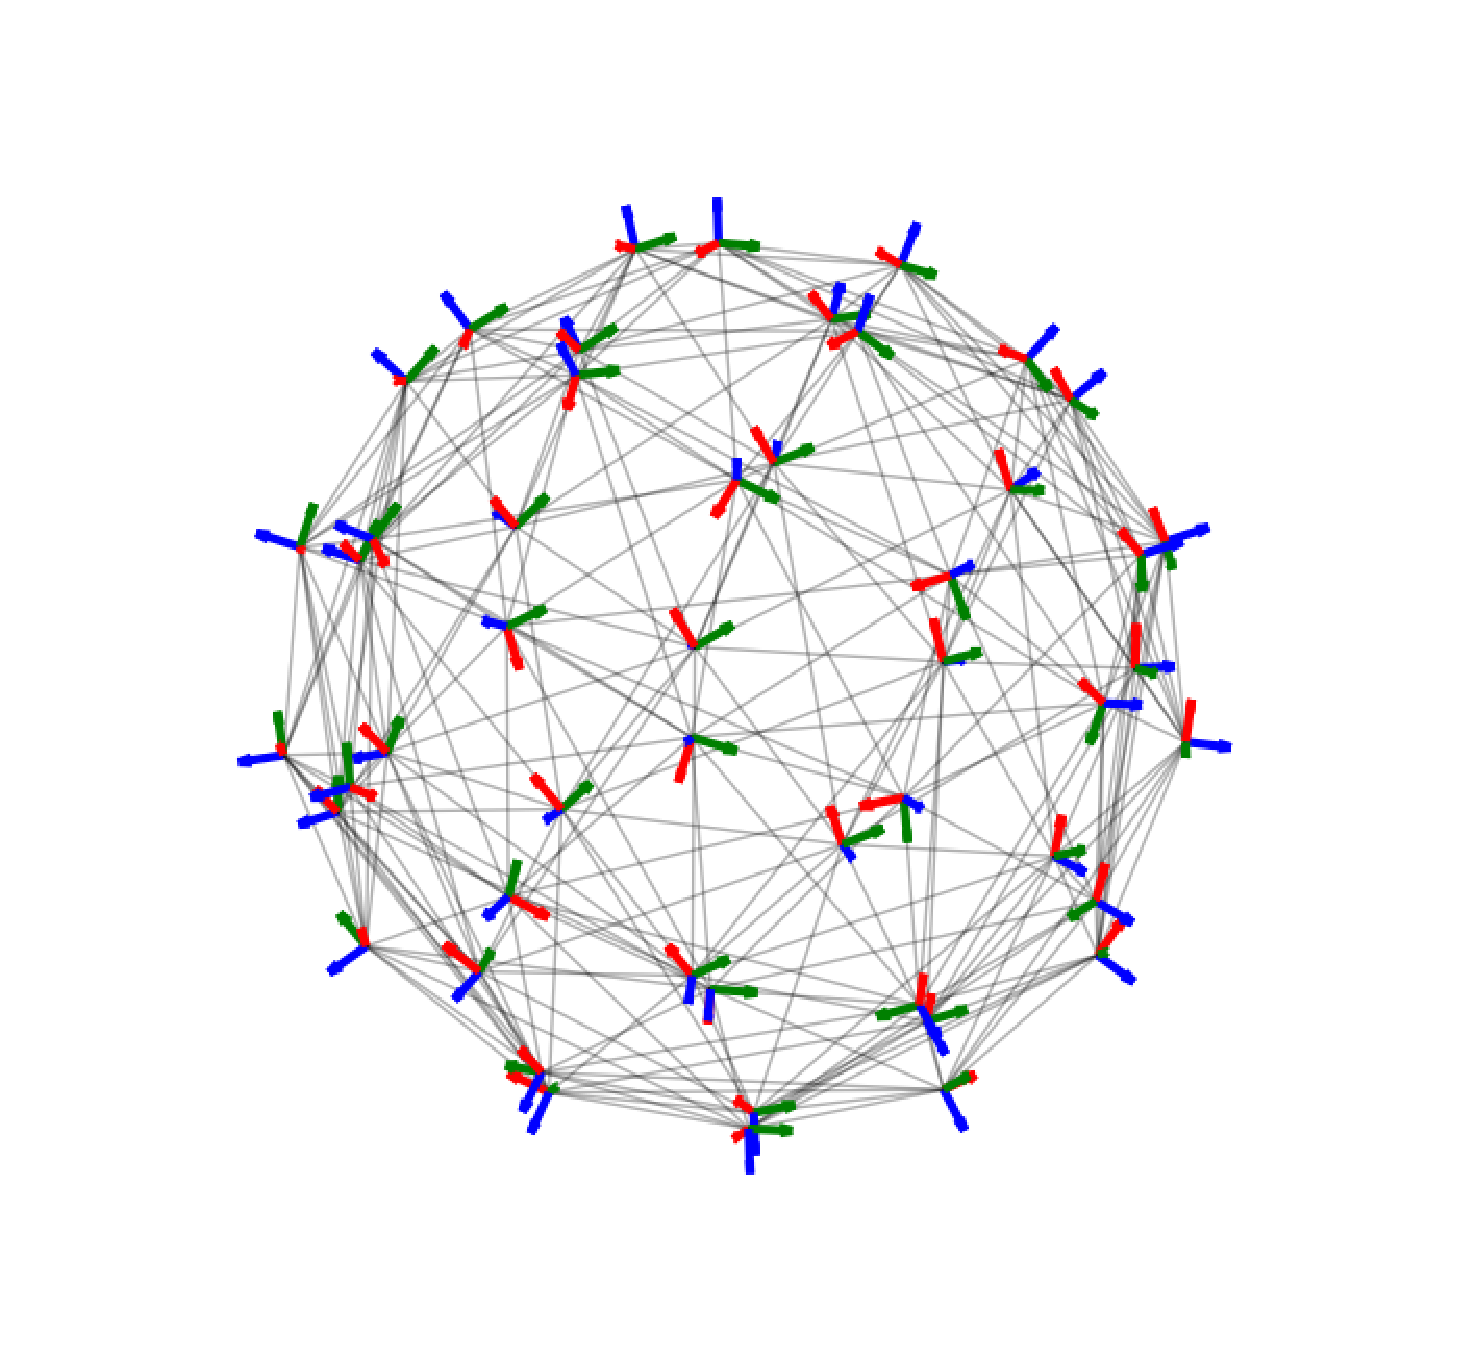
\includegraphics[width=0.45\linewidth]{fig/gt_graph.eps}%
    }
    \hfill
    \subfloat[DPGO result in an outlier environment (40\% incorrect edges)\label{fig:messy_graph}]{%
        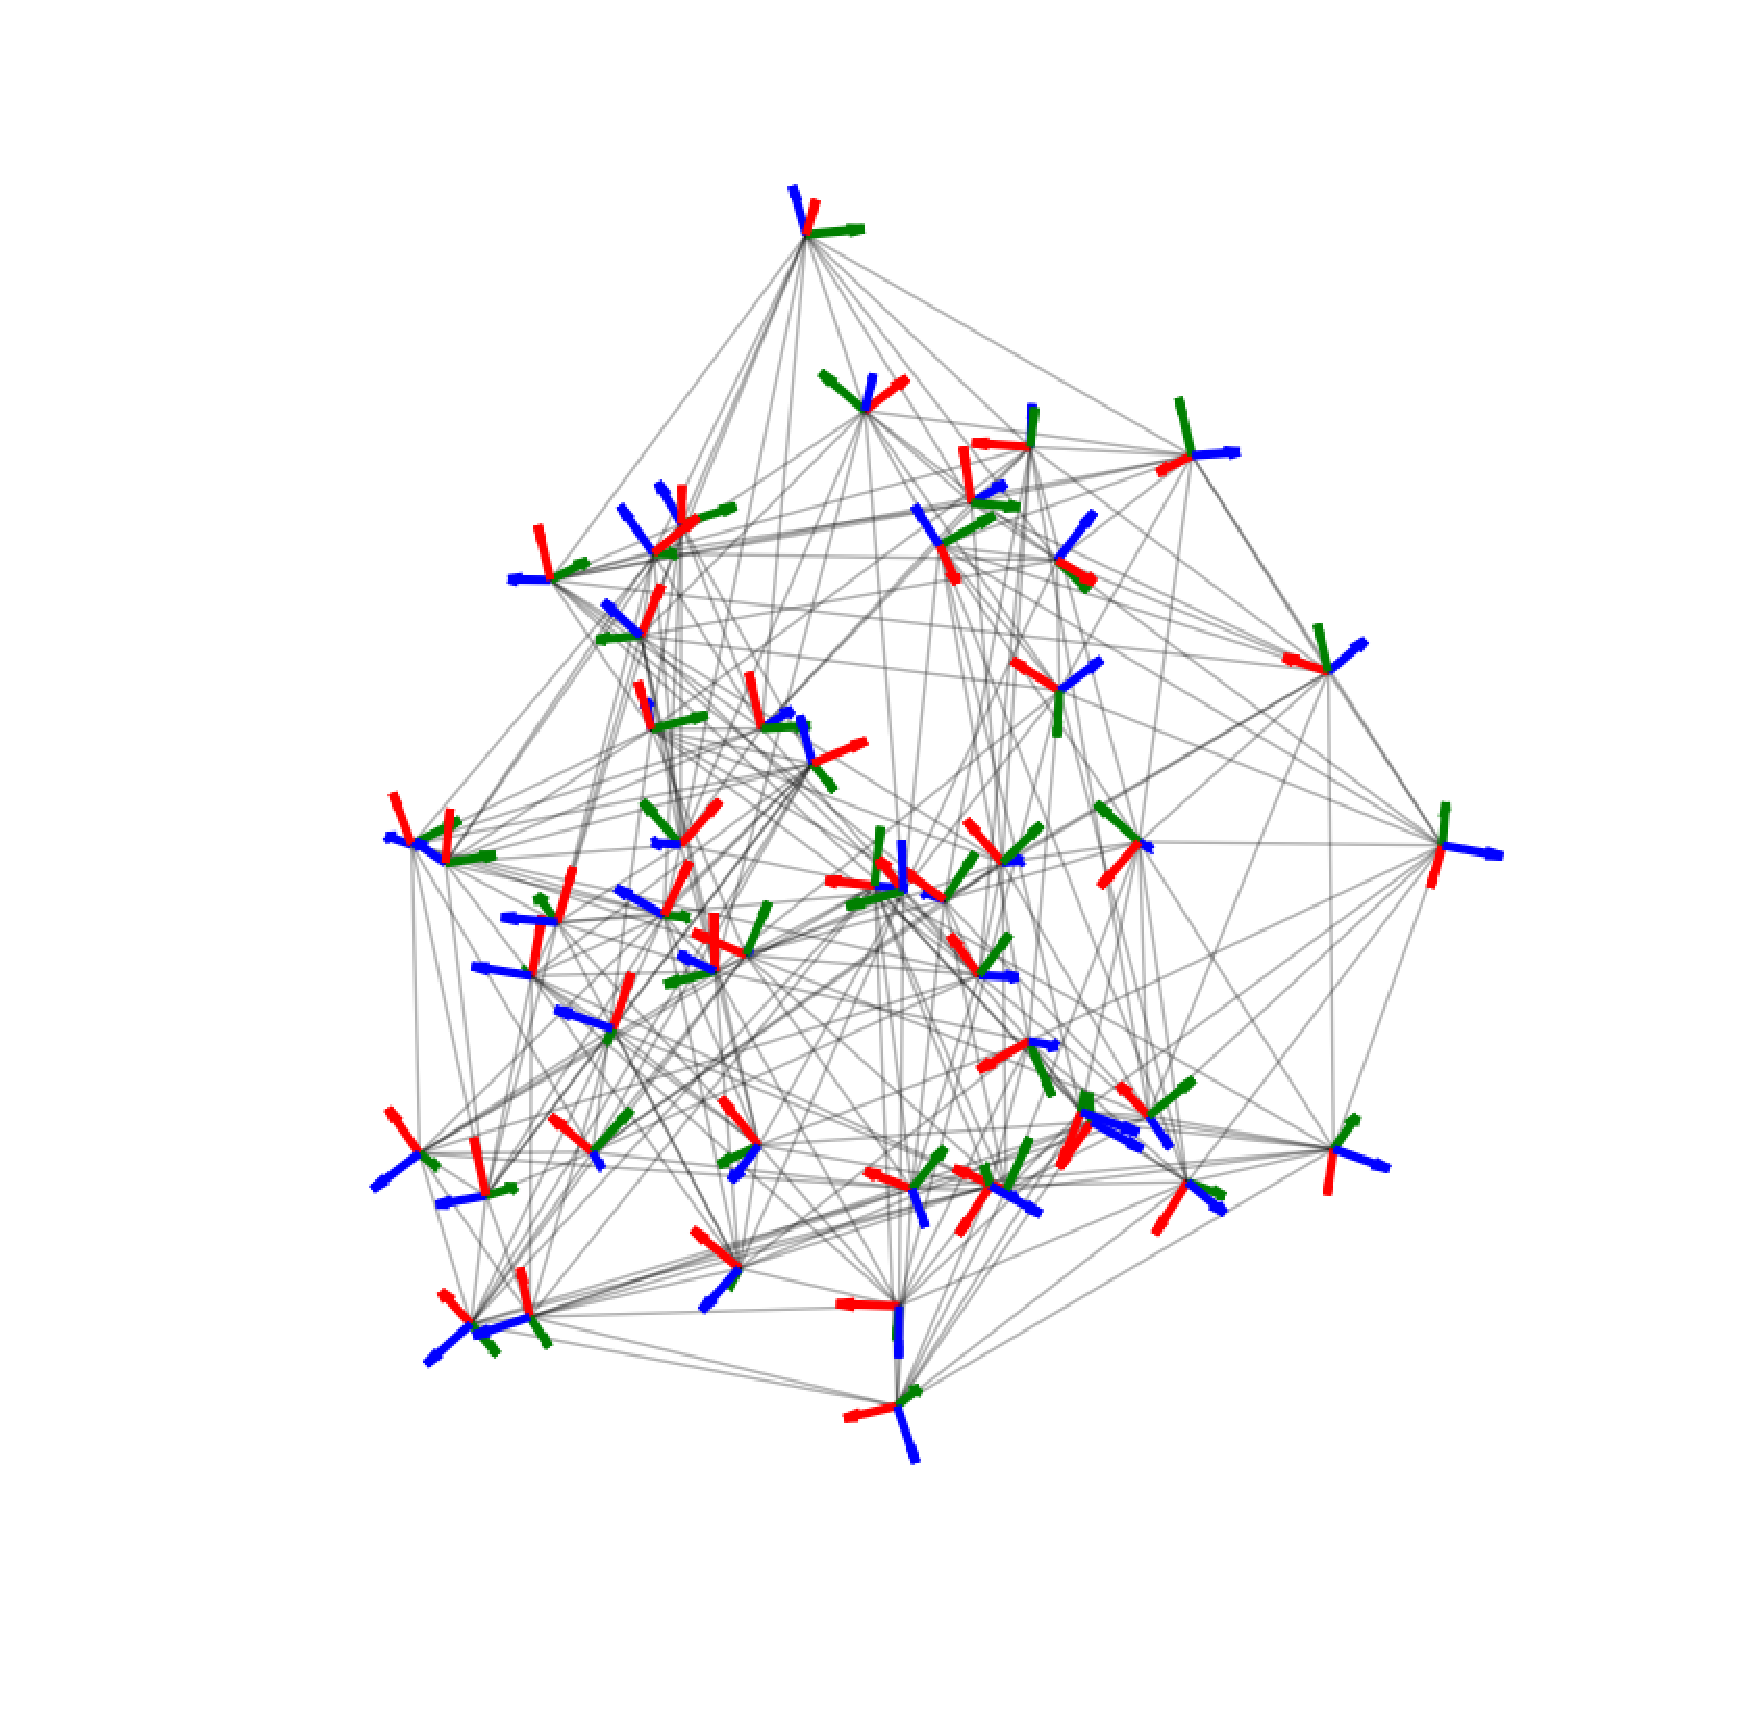
\includegraphics[width=0.45\linewidth]{fig/messy_graph.eps}%
    }
    \caption{Comparison of ground truth and DPGO performance in an outlier-rich environment.}
    \label{fig:gt_messy_comparison}
\end{figure}

In this section, we further evaluate the performance of the proposed method in environments with and without outliers.
We compare our method with the proposed method using Gauss-Newton optimization, and Distributed Certifiably Correct Pose-Graph Optimization (DPGO)~\cite{Tian2021}.

\subsection{Environment without Outliers}
\label{subsec:eval_no_outliers}

Figures~\ref{fig:no_outliers_graphs_1} and \ref{fig:no_outliers_graphs_last} show the pose graphs before and after optimization, respectively.
Figure~\ref{fig:no_outliers_edge_errors} shows the time transition of the edge cost $c_{ij}$, and Figure~\ref{fig:no_outliers_particle_variances} shows the time transition of the particle variance for each agent.
Specifically, Figure~\ref{fig:no_outliers_edge_errors} displays the range (shaded area) between the minimum and maximum costs across all connected edges, along with their mean value.
Figure~\ref{fig:no_outliers_particle_variances} similarly shows the range (shaded area) of particle variances across all agents, and their mean value.

\begin{figure}[H]
    \centering
    \subfloat[Before optimization\label{fig:no_outliers_graphs_1}]{%
        \includegraphics[width=0.45\linewidth]{fig/graph_temp_step_1.eps}%
    }
    \hfill
    \subfloat[After optimization\label{fig:no_outliers_graphs_last}]{%
        \includegraphics[width=0.45\linewidth]{fig/graph_temp_step_last.eps}%
    }
    \\
    \subfloat[Edge errors $c_{ij}$\label{fig:no_outliers_edge_errors}]{%
        \includegraphics[width=0.45\linewidth]{fig/edge_errors_temp.eps}%
    }
    \hfill
    \subfloat[Particle variances\label{fig:no_outliers_particle_variances}]{%
        \includegraphics[width=0.45\linewidth]{fig/particle_variances_temp.eps}%
    }
    \caption{Evaluation in an environment without outliers.}
    \label{fig:eval_no_outliers}
\end{figure}

\subsection{Environment with Outliers}
\label{subsec:eval_with_outliers}

In this subsection, we evaluate the performance in an environment with outliers. In this outlier validation (corresponding to Figure~\ref{fig:eval_with_outliers}), incorrect edges are selected at a rate of 0.3 in each step.
Figures~\ref{fig:with_outliers_graphs_1} and \ref{fig:with_outliers_graphs_last} show the pose graphs before and after optimization in an environment with outliers.
Figure~\ref{fig:with_outliers_edge_errors} shows the time transition of the edge cost $c_{ij}$, and Figure~\ref{fig:with_outliers_particle_variances} shows the time transition of the particle variance for each agent.
Specifically, Figure~\ref{fig:with_outliers_edge_errors} displays the range (shaded area) between the minimum and maximum costs across all connected edges, along with their mean value. It shows that although errors occur, they do not diverge and maintain a certain level.
Figure~\ref{fig:with_outliers_particle_variances} similarly shows the range (shaded area) of particle variances across all agents, and their mean value, indicating that outliers cause an increase in particle variance.

\begin{figure}[H]
    \centering
    \subfloat[Before optimization\label{fig:with_outliers_graphs_1}]{%
        \includegraphics[width=0.45\linewidth]{fig/graph_temp2_step_1.eps}%
    }
    \hfill
    \subfloat[After optimization\label{fig:with_outliers_graphs_last}]{%
        \includegraphics[width=0.45\linewidth]{fig/graph_temp2_step_last.eps}%
    }
    \\
    \subfloat[Edge errors $c_{ij}$\label{fig:with_outliers_edge_errors}]{%
        \includegraphics[width=0.45\linewidth]{fig/edge_errors_temp2.eps}%
    }
    \hfill
    \subfloat[Particle variances\label{fig:with_outliers_particle_variances}]{%
        \includegraphics[width=0.45\linewidth]{fig/particle_variances_temp2.eps}%
    }
    \caption{Evaluation in an environment with outliers.}
    \label{fig:eval_with_outliers}
\end{figure}

% \subsection{Benchmark Results}
% \label{subsec:benchmark_results}

In the benchmark comparisons, for DPGO, an optimization problem with incorrectly selected edges based on each outlier ratio is solved. For the proposed method (ASP-PGF), edges are randomly misselected at each of the 50 steps based on the outlier ratio. As demonstrated in our experiments, the algorithm consistently converges to a KKT point (as proven in Theorem 4.1) within 50 iterations in our 20-agent, 1000-particle scenario, confirming the theoretical guarantees.

Table~\ref{tab:benchmark_results} summarizes the performance metrics for each method.
As the outlier ratio increases, the filtering-based proposed method (ASP-PGF) surpasses the accuracy of optimization-based methods like DPGO.

\begin{table}[H]
  \centering
  \caption{Benchmark Results (Single Metric)}
  \label{tab:benchmark_results}
  \begin{tabular}{@{}lccc@{}}
    \toprule
    Environment & DPGO~\cite{Tian2021} & ASP-PGF(GN) \\
    \midrule
    Without Outliers & \textbf{1.10}\times 10^{-11} & 0.026 \\
    Outlier Ratio 0.2 & \textbf{0.216} & 0.591 \\
    Outlier Ratio 0.4 & 0.902 & \textbf{0.742} \\
    \bottomrule
  \end{tabular}
\end{table}

\section{Conclusion}
\label{sec:conclusion}

This paper introduced ASP-PGF, a novel framework for multi-agent pose graph filtering that addresses ambiguity and outliers by integrating distributed optimization (ADMM) with non-parametric Bayesian inference (SVGD). We formulated PGF as approximating the full posterior via KL divergence minimization, enabling distributed computation where agents update local particle-based beliefs using SVGD, achieving consensus through ADMM.

The main contributions are:
\begin{enumerate}
    \item \textbf{Distributed Non-Parametric Posterior Estimation via ADMM and SVGD Integration:} We formulate multi-robot PGF as a distributed posterior-estimation problem, decomposing it into local SVGD updates that exchange only summary statistics through ADMM.
    Convergence to a KKT point is rigorously proved in Theorem 4.1, and the algorithm reaches this point within 50 iterations in a 20-agent, 2000-particle scenario.
    \item \textbf{Robust Multimodal Uncertainty Handling:} The particle-based Bayesian representation preserves non-Gaussian, multimodal structure and down-weights outliers automatically.
    In simulation, even with a 40\% outlier ratio the mean error remains 0.742, outperforming the state-of-the-art DPGO (0.902); the advantage widens as outlier rates increase.
\end{enumerate}
ASP-PGF advances robust, informative multi-agent SLAM. Future work includes real-world validation, adaptive parameter strategies, front-end integration, and further SE(3) convergence analysis, particularly addressing the challenges posed by the non-convex nature of the SE(3) manifold.

\begin{thebibliography}{99}

\bibitem{Cadena2016}
C. Cadena, L. Carlone, H. Carrillo, Y. Latif, D. Scaramuzza, J. Neira, I. Reid, and J. J. Leonard, ``Past, Present, and Future of Simultaneous Localization and Mapping: Toward the Robust-Perception Age,'' {\it {IEEE} Trans. Robotics}, Vol. 32, No. 6, pp. 1309--1332, 2016.

\bibitem{Grisetti2010}
G. Grisetti, R. Kümmerle, C. Stachniss, and W. Burgard, ``A Tutorial on Graph-Based {SLAM},'' {\it IEEE Intell. Transport. Syst. Mag.}, Vol. 2, No. 4, pp. 31--43, 2010.

\bibitem{Kuemmerle2011}
R. Kümmerle, G. Grisetti, H. Strasdat, K. Konolige, and W. Burgard, ``{g2o}: A General Framework for Graph Optimization,'' {\it Proc. {IEEE} Int. Conf. Robot. Autom. ({ICRA})}, pp. 3607--3613, 2011.

\bibitem{Kaess2012}
M. Kaess, H. Johannsson, R. Roberts, V. Ila, J. J. Leonard, and F. Dellaert, ``{iSAM2}: Incremental Smoothing and Mapping Using the Bayes Tree,'' {\it Int. J. Robotics Research}, Vol. 31, No. 2, pp. 216--235, 2012.

\bibitem{Cunningham2013}
A. Cunningham, V. Indelman, and F. Dellaert, ``{DDF-SAM} 2.0: Consistent Distributed Smoothing and Mapping,'' {\it Proc. {IEEE} Int. Conf. Robot. Autom. ({ICRA})}, pp. 5220--5227, 2013.

\bibitem{Choudhary2015}
S. Choudhary, L. Carlone, H. I. Christensen, and F. Dellaert, ``Exactly Sparse Memory Efficient {SLAM} using the Multi-Block Alternating Direction Method of Multipliers,'' {\it Proc. {IEEE/RSJ} Int. Conf. Intelligent Robots and Systems ({IROS})}, pp. 1349--1356, 2015.

\bibitem{Boyd2011}
S. Boyd, N. Parikh, E. Chu, B. Peleato, and J. Eckstein, ``Distributed Optimization and Statistical Learning via the Alternating Direction Method of Multipliers,'' {\it Found. Trends Mach. Learn.}, Vol. 3, No. 1, pp. 1--122, 2011.

\bibitem{Choudhary2017}
S. Choudhary, L. Carlone, J. Nieto, J. Rogers, H. I. Christensen, and F. Dellaert, ``Distributed Mapping with Privacy and Communication Constraints: Lightweight Algorithms and Object-Based Models,'' {\it Int. J. Robotics Research}, Vol. 36, No. 12, pp. 1286--1311, 2017.

\bibitem{Lajoie2020}
P.-Y. Lajoie, Y. Hu, Y. Chang, B. Ramtoula, and L. Carlone, ``{DOOR-SLAM}: Distributed, Online, and Outlier Resilient {SLAM} for Robotic Teams,'' {\it {IEEE} Robotics Autom. Lett.}, Vol. 5, No. 2, pp. 1656--1663, 2020.


\bibitem{Montemerlo2002}
M. Montemerlo, S. Thrun, D. Koller, and B. Wegbreit, ``{FastSLAM}: A Factored Solution to the Simultaneous Localization and Mapping Problem,'' {\it Proc. 18th Nat. Conf. on Artificial Intelligence ({AAAI})}, pp. 593--598, 2002.

\bibitem{Liu2016}
Q. Liu and D. Wang, ``Stein Variational Gradient Descent: A General Purpose Bayesian Inference Algorithm,'' {\it Proc. 30th Conf. Neural Information Processing Systems ({NIPS})}, pp. 2370--2378, 2016.

\bibitem{Pavlasek2023}
J. Pavlasek, J. J. Z. Mah, R. Xu, O. C. Jenkins, and F. Ramos, ``Stein Variational Belief Propagation for Multi-Robot Coordination,'' {\it arXiv:2311.16916}, 2023.

\bibitem{Koide2024MegaParticles}
K. Koide, S. Oishi, M. Yokozuka, and A. Banno, ``MegaParticles: Range-based 6-DoF Monte Carlo Localization with GPU-Accelerated Stein Particle Filter,'' {\it Proc. {IEEE} Int. Conf. Robot. Autom. ({ICRA})}, 2024.

\bibitem{Cao2024}
H. Cao, S. Shreedharan, and N. Atanasov, ``Multi-Robot Object {SLAM} Using Distributed Variational Inference,'' {\it arXiv:2404.18331}, 2024.

\bibitem{Agarwal2013}
P. Agarwal, G. D. Tipaldi, L. Spinello, C. Stachniss, and W. Burgard, ``Robust Map Optimization Using Dynamic Covariance Scaling,'' {\it Proc. {IEEE} Int. Conf. Robot. Autom. ({ICRA})}, pp. 62--69, 2013.

\bibitem{Sunderhauf2012}
N. Sünderhauf and P. Protzel, ``Switchable Constraints for Robust Pose Graph {SLAM},'' {\it Proc. {IEEE/RSJ} Int. Conf. Intelligent Robots and Systems ({IROS})}, pp. 1879--1884, 2012.

\bibitem{Olson2013}
E. Olson and P. Agarwal, ``Inference on Networks of Mixtures for Robust Robot Mapping,'' {\it Int. J. Robotics Research}, Vol. 32, No. 7, pp. 826--840, 2013.

\bibitem{Yang2020}
H. Yang, P. Antonante, V. Tzoumas, and L. Carlone, ``Graduated Non-Convexity for Robust Spatial Perception: From Non-Minimal Solvers to Global Outlier Rejection,'' {\it {IEEE} Robotics Autom. Lett.}, Vol. 5, No. 2, pp. 1127--1134, 2020.

\bibitem{Latif2013}
Y. Latif, C. Cadena, and J. Neira, ``Robust Loop Closing Over Time for Pose Graph {SLAM},'' {\it Int. J. Robotics Research}, Vol. 32, No. 14, pp. 1611--1626, 2013.

\bibitem{Mangelson2018}
J. G. Mangelson, D. Dominic, R. M. Eustice, and R. Vasudevan, ``Pairwise Consistent Measurement Set Maximization for Robust Multi-Robot Map Merging,'' {\it Proc. {IEEE} Int. Conf. Robot. Autom. ({ICRA})}, pp. 2916--2923, 2018.

\bibitem{Hong2016}
M. Hong, Z.-Q. Luo, and M. Razaviyayn, ``Convergence Analysis of Alternating Direction Method of Multipliers for a Family of Nonconvex Problems,'' {\it SIAM Journal on Optimization}, Vol. 26, No. 1, pp. 337--364, 2016.

\bibitem{Wang2019}
Y. Wang, W. Yin, and J. Zeng, ``Global Convergence of ADMM in Nonconvex Nonsmooth Optimization,'' {\it Journal of Scientific Computing}, Vol. 78, No. 1, pp. 29--61, 2019.

\bibitem{Blanco2012ATO}
J.-L. Blanco, ``A tutorial on SE(3) transformation parameterizations and on-manifold optimization,'' {\it MAPIR Group Technical report \#012010}, University of Malaga, 2010 (Updated 2012).

\bibitem{Tian2021}
Y. Tian, K. Khosoussi, D. M. Rosen, and J. P. How, ``Distributed Certifiably Correct Pose-Graph Optimization,'' {\it {IEEE} Trans. Robotics}, Vol. 37, No. 6, pp. 2137--2156, 2021.

\end{thebibliography}


%\processdelayedfloats %%% See above for an explanation of why this command might be needed here.


\end{document}
